
% v2-acmsmall-sample.tex, dated March 6 2012
% This is a sample file for ACM small trim journals
%
% Compilation using 'acmsmall.cls' - version 1.3 (March 2012), Aptara Inc.
% (c) 2010 Association for Computing Machinery (ACM)
%
% Questions/Suggestions/Feedback should be addressed to => "acmtexsupport@aptaracorp.com".
% Users can also go through the FAQs available on the journal's submission webpage.
%
% Steps to compile: latex, bibtex, latex latex
%
% For tracking purposes => this is v1.3 - March 2012
\documentclass[prodmode,acmtecs]{acmsmall} % Aptara syntax
\usepackage[spanish,polish]{babel}
\usepackage[T1]{fontenc}
\usepackage{fancyvrb}
\usepackage{graphicx,hyperref}
\newcommand\cutout[1]{}


\usepackage[table]{xcolor}
\usepackage[utf8]{inputenc}
\usepackage[parfill]{parskip}
\usepackage{tabulary}
\PassOptionsToPackage{hyphens}{url}
\usepackage{hyperref}    
\usepackage[capitalize]{cleveref}


% Metadata Information
% !!! TODO: SET THESE VALUES !!!
\acmVolume{0}
\acmNumber{0}
\acmArticle{CFP}
\acmYear{0}
\acmMonth{0}

\newcounter{colstart}
\setcounter{page}{4}

\RecustomVerbatimCommand{\VerbatimInput}{VerbatimInput}%
{
%fontsize=\footnotesize,
fontfamily=\rmdefault
}


\newcommand{\UnderscoreCommands}{%\do\verbatiminput%
\do\citeNP \do\citeA \do\citeANP \do\citeN \do\shortcite%
\do\shortciteNP \do\shortciteA \do\shortciteANP \do\shortciteN%
\do\citeyear \do\citeyearNP%
}

\usepackage[strings]{underscore}



% Document starts
\begin{document}


\setcounter{colstart}{\thepage}

\acmArticle{CFP}
\title{{\huge\sc SIGLOG Monthly 245}

 January 2024}
\author{DAVID PURSER\affil{University of Liverpool, UK}
ELLI ANASTASIADI\affil{Uppsala University, Sweden}
\vspace*{-2.6cm}\begin{flushright}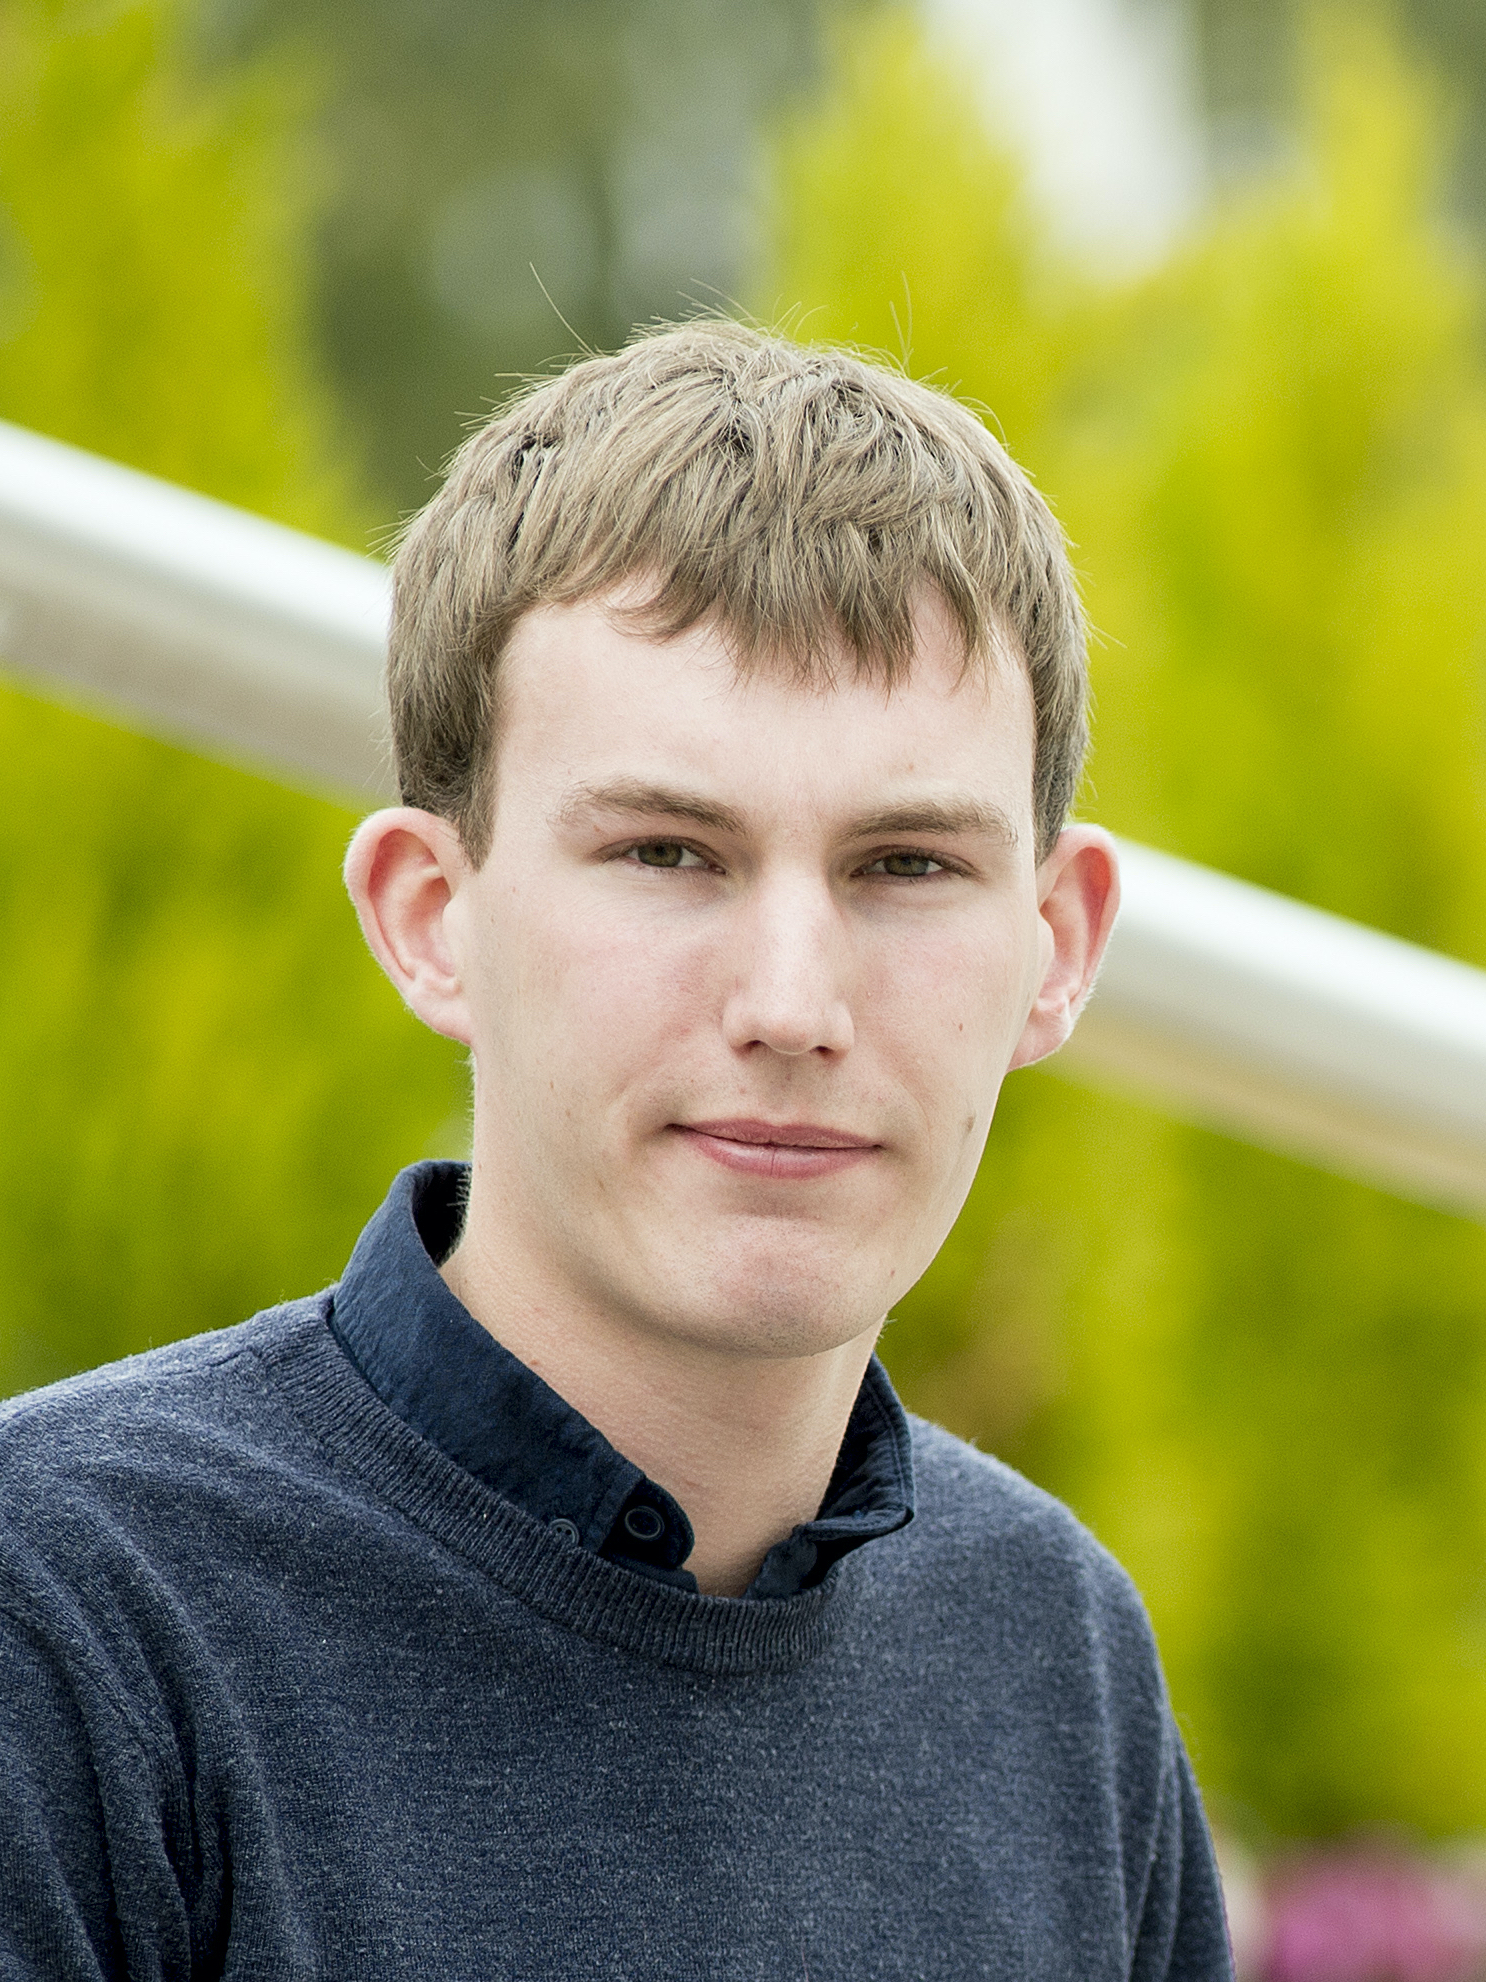
\includegraphics[height=35mm]{dp}\ 
\includegraphics[height=35mm]{ea}\end{flushright}
}



\begin{abstract}
January 2024 edition of SIGLOG Monthly, featuring deadlines, calls and community announcements.
\end{abstract}


\maketitlee

\href{https://lics.siglog.org/newsletters/}{Past Issues}
 - 
\href{https://lics.siglog.org/newsletters/inst.html}{How to submit an announcement}
\section{Table of Content}\begin{itemize}\item DEADLINES (\cref{deadlines}) 
 
\item SIGLOG MATTERS 
 
\begin{itemize}\item LICS 2024 (\cref{LICS2024})
\end{itemize} 
\item CALLS 
 
\begin{itemize}\item COORDINATION 2024 (CALL FOR PAPERS) (\cref{COORDINATION2024})
\item CiE 2024 (CALL FOR PAPERS) (\cref{CiE2024})
\item ACT / MFPS 2024 (CALL FOR PAPERS) (\cref{ACTMFPS2024})
\end{itemize} 
\item JOB ANNOUNCEMENTS 
 
\begin{itemize}\item PHD POSITION IN MARSEILLE (\cref{PHDPOSITIONINMARSEILLE})
\item PhD or Postdoc position at TU Wien, Project TAIGER (\cref{PhDorPostdocpositionatTUWienProjectTAIGER})
\end{itemize} 
\end{itemize}\section{Deadlines}\label{deadlines}\rowcolors{1}{white}{gray!25}\begin{tabulary}{\linewidth}{LL}DEON2023:  & Jan 07, 2024 (Paper) \\
SPIN 2024:  & Jan 15, 2024 (Submissions) \\
CAV 2024:  & Jan 19, 2024 (Paper), Mar 01, 2024 (CAV Award Nomination deadline) \\
LICS 2024:  & Jan 21, 2024 (Titles and Short Abstracts), Jan 26, 2024 (Full Papers Due) \\
IJCAR 2024:  & Jan 29, 2024 (Abstract, extended), Feb 05, 2024 (Paper, extended) \\
COORDINATION 2024:  & Feb 02, 2024 (Abstract), Feb 09, 2024 (Paper) \\
FSCD 2024:  & Feb 05, 2024 (Abstract), Feb 12, 2024 (Paper) \\
CiE 2024:  & Feb 10, 2024 (Article), May 15, 2024 (Informal presentations), Feb 10, 2024 (Article) \\
ICALP 2024:  & Feb 14, 2024 (Paper) \\
ICGT 2024:  & Feb 27, 2024 (Abstract), Mar 05, 2024 (Paper) \\
PHD POSITION IN MARSEILLE:  & Feb 28, 2024 (Application deadline) \\
AiML 2024:  & Mar 08, 2024 (Abstract), Mar 15, 2024 (Full papers) \\
ACT / MFPS 2024:  & Mar 29, 2024 (Conference) \\
\end{tabulary}
\section{LICS 2024: Thirty-Ninth Annual ACM/IEEE Symposium on}\label{LICS2024}LOGIC IN COMPUTER SCIENCE 

  Tallinn, July 2024\\ 
  \href{https://lics.siglog.org/lics24}{https://lics.siglog.org/lics24}\\ 
CALL FOR PAPERS 

\begin{itemize}\item  SCOPE 
 
  The LICS Symposium is an annual international forum on theoretical and practical topics in computer science that relate to logic, broadly construed. We invite submissions on topics that fit under that rubric. Suggested, but not exclusive, topics of interest include: automata theory, automated deduction, categorical models and logics, concurrency and distributed computation, constraint programming, constructive mathematics, database theory, decision procedures, description logics, domain theory, finite model theory, formal aspects of program analysis, formal methods, foundations of computability, foundations of probabilistic, real-time and hybrid systems, games and logic, higher-order logic, knowledge representation and reasoning, lambda and combinatory calculi, linear logic, logic programming, logical aspects of AI, logical aspects of bioinformatics, logical aspects of computational complexity, logical aspects of quantum computation, logical frameworks, logics of programs, modal and temporal logics, model checking, process calculi, programming language semantics, proof theory, reasoning about security and privacy, rewriting, type systems, type theory, and verification. 
 
\item  IMPORTANT DATES FOR PAPERS 
 
  Authors are required to submit a paper title and a short abstract of about 100 words in advance of submitting the extended abstract of the paper. The exact deadline time on these dates is anywhere on earth (AoE). 
 
\rowcolors{1}{white}{gray!25}\begin{tabulary}{\linewidth}{LL}Titles and Short Abstracts Due:  & Jan 21, 2024 \\
Full Papers Due:  & Jan 26, 2024 \\
Author Feedback/Rebuttal Period:  & Mar 18-23, 2024 \\
Author Notification:  & Apr 15, 2024 \\
Conference:  & Jul 8-12, 2024 \\
\end{tabulary}
 
  Submission deadlines are firm; late submissions will not be considered. All submissions will be electronic via easychair. 
 
\item  PAPER SUBMISSION INSTRUCTIONS 
 
  Submissions should use ACM SIGCONF Proceedings 2-column 10pt format and may be at most 12 pages, excluding references. Latex style files and further submission information is at \href{https://lics.siglog.org/lics24/cfp.php}{https://lics.siglog.org/lics24/cfp.php}.  
 
  LICS 2024 will use a lightweight double-blind reviewing process. Please see the website for further details and requirements from the double-blind process. 
 
  The official publication date may differ from the first day of the conference. The official publication date may affect the deadline for any patent filings related to published work. We will clarify the official publication date in due course. 
 
\end{itemize}\section{COORDINATION 2024: 26th International Conference on Coordination Models and Languages}\label{COORDINATION2024}  June 18-20, 2024 University of Groningen, The Netherlands\\ 
  \href{https://www.discotec.org/2024/coordination}{https://www.discotec.org/2024/coordination}\\ 
CALL FOR PAPERS 

\begin{itemize}\item  SCOPE 
 
  Modern information systems rely increasingly on combining concurrent, distributed, mobile, adaptive, reconfigurable, and heterogeneous components. New models, architectures, languages, and verification techniques are necessary to cope with the complexity induced by the demands of today's software development. Coordination languages have emerged as a successful approach, in that they provide abstractions that cleanly separate behaviour from communication, therefore increasing modularity, simplifying reasoning, and ultimately enhancing software development. Building on the success of the previous editions, this conference provides a well-established forum for the growing community of researchers interested in models, languages, architectures, and implementation techniques for coordination. 
 
\item  TOPICS 
 
\begin{itemize}\item  Theoretical models and foundations for coordination: component composition, concurrency, distribution, mobility; dynamic, spatial and probabilistic aspects of coordination; logic, types, semantics. 
\item  Coordination of multi-agent and collective systems: models, languages, infrastructures, self-adaptation, self-organisation, distributed solving, collective intelligence and emerging behaviour. 
\item  Coordination and modern distributed computing: web services, microservices, peer-to-peer networks, grid computing, context-awareness, ubiquitous computing, mobile computing, reversible computing. 
\item  Session-based programming: models, languages, behavioural types, and tools. 
\item  Models, languages, verification techniques, and tools for interacting smart contracts and (blockchain-based) decentralised applications. 
\item  Languages, methodologies, and tools for secure coordination. 
\item  Cybersecurity aspects of coordinated systems, coordinated approaches to cybersecurity. 
\item  Nature and bio-inspired approaches to coordination. 
\item  Specification, refinement, and analysis of architectures: patterns and styles, verification of functional and non-functional properties, including performance and security aspects. 
\item  Dynamic software architectures: distributed mobile code, configuration, reconfiguration, networked computing, parallel, high-performance and cloud computing. 
\item  Coordination platforms for infrastructures of emergent new application domains, like IoT, fog-, and edge-computing. 
\item  Programming methodologies, languages, middleware, tools, and environments for the development and verification of coordinated applications, including DevOps approaches. 
\item  Coordination in business process management: coordination models for business process management, process mining techniques and tools for coordination models. 
\item  Industrial relevance of coordination and software architectures: programming in the large, domain-specific software architectures and coordination models, industry-driven efforts in coordination and case studies. 
\item  Interdisciplinary aspects of coordination.
\end{itemize} 
\item  INVITED SPEAKER  
 
  Marieke Huisman, University of Twente, The Netherlands 
 
\item  IMPORTANT DATES (AoE)  
 
\rowcolors{1}{white}{gray!25}\begin{tabulary}{\linewidth}{LL}Abstract submission:  & Feb 02, 2024 \\
Paper submission:  & Feb 09, 2024 \\
Paper notification:  & Mar 29, 2024 \\
Camera-ready:  & Apr 24, 2024 \\
\end{tabulary}
 
\item  SUBMISSION 
 
  Please see full call for submission information: \href{https://www.discotec.org/2024/coordination}{https://www.discotec.org/2024/coordination} 
 
\item  ARTEFACTS 
 
  To improve and reward reproducibility and to give more visibility and credit to the effort of tool developers in the COORDINATION community, authors of submitted papers are invited to submit publicly available artefacts (using permanent repositories such as Software Heritage, Zenodo, etc.), which will be associated with their paper for evaluation. Based on the result of the artefact evaluation, one or more badges may be applied to a paper. Specifically, COORDINATION uses the EAPLS badging scheme [2], which in its own turn is based on and consistent with the ACM initiative. 
 
  Artefact submission is mandatory for tool papers and the result of the artefact evaluation will be considered in the tool paper's acceptance decision. Instead, artefact submission is optional for all the other paper categories and the result of the artefact evaluation will not affect the paper's acceptance decision but may affect the best paper selection. 
 
\rowcolors{1}{white}{gray!25}\begin{tabulary}{\linewidth}{LL}Artefact submission:  & Feb 29, 2024 \\
Problem reports from reviewers:  & Mar 08, 2024 \\
Authors' response to reviewers:  & Mar 15, 2024 \\
Artefact notification:  & Mar 29, 2024 \\
\end{tabulary}
 
\item  SPECIAL ISSUES 
 
  After the conference, accepted papers (except for tool papers) selected from COORDINATION and FORTE programmes will be invited to a special issue of the Logical Methods in Computer Science journal. The paper submission deadline is planned for October/November 2024, while the notifications for the first round of reviews around February 2025. Selected accepted tool papers, instead, will be invited to a special issue of a reputable journal with a track dedicated to software, like the Journal of Science of Computer Programming's Software Track. 
 
\end{itemize}\section{CiE 2024: Computability in Europe 2024}\label{CiE2024}  Twenty years of theoretical and practical synergies\\ 
  July 08-12, 2024 Amsterdam, The Netherlands\\ 
  \href{https://events.illc.uva.nl/CiE/CiE2024/}{https://events.illc.uva.nl/CiE/CiE2024/}\\ 
  Submission link: \href{https://equinocs.springernature.com/service/CiE2024}{https://equinocs.springernature.com/service/CiE2024}\\ 
CALL FOR PAPERS 

\begin{itemize}\item  IMPORTANT DATES:  (AOE) 
 
\rowcolors{1}{white}{gray!25}\begin{tabulary}{\linewidth}{LL}Article submission:  & Feb 10, 2024 \\
Notification of acceptance:  & Apr 20, 2024 \\
Final versions due:  & May 01, 2024 \\
Deadline for informal presentations submission:  & May 15, 2024 \\
Early registration before:  & May 20, 2024 \\
Conference:  & Jul 08-12, 2024 \\
\end{tabulary}
 
  The notifications of acceptance for informal presentations will be sent a few days after submission. 
 
\item  GENERAL INFORMATION 
 
  CiE 2024 will be an anniversary event. It is the 20th conference organized by CiE (Computability in Europe), in the same place as the first edition, Amsterdam. 
 
  CiE is a European association of mathematicians, logicians, computer scientists, philosophers, physicists and others interested in new developments in computability and their underlying significance for the real world. 
 
\item  TUTORIAL SPEAKERS 
 
\begin{itemize}\item  Matthew Harrison-Trainor (University of Illinois Chicago)
\item  Sonja Smets (University of Amsterdam)
\end{itemize} 
\item  INVITED SPEAKERS 
 
\begin{itemize}\item  Arnold Beckmann (Swansea University)
\item  Rod Downey (Victoria University of Wellington)
\item  Elvira Mayordomo (University of Zaragoza)
\item  Alexandre Miquel (Universidad de la República)
\item  Monika Seisenberger (Swansea University)
\item  Mariya Soskova (University of Wisconsin–Madison)
\end{itemize} 
\item  SPECIAL SESSIONS 
 
  There will be 6 special sessions: 
 
\begin{itemize}\item  Computable aspects of symbolic dynamics and tilings (chairs: Benjamin Hellouin and Ilkka Torma)
\item  Algorithmic randomness and Kolmogorov complexity session (chairs: Rupert Hölzl abd Denis Hirschfeldt)
\item  Quantum Computation (chairs: Delaram Kahrobaei and Mehrnoosh Sadrzadeh)
\item  History and Philosophy of Computing (HaPoC) (chairs: Ekaterina Koubychkina and Marianna Girlando)
\item  Bio-inspired Computation (BiC) (chairs: Gianluca Della Vedova and Jasmijn Baaijens)
\item  Computable Structure Theory (chairs: Stefan Vatev and Ekaterina Fokina)
\end{itemize} 
\item  CONFERENCE TOPICS 
 
  The CiE conferences serve as an interdisciplinary forum for research in all aspects of computability, foundations of computer science, logic, and theoretical computer science, as well as the interplay of these areas with practical issues in computer science and with other disciplines such as biology, mathematics, philosophy, or physics. 
 
\item  PAPER SUBMISSION 
 
  THE PROGRAM COMMITTEE cordially invites all researchers, European and non-European, to submit their papers in all areas related to the above for presentation at the conference and inclusion in the proceedings of CiE 2024 at \href{https://equinocs.springernature.com/service/CiE2024}{https://equinocs.springernature.com/service/CiE2024} 
 
\item  CONFERENCE PROCEEDINGS 
 
  Papers to be considered in the conferences proceedings must be submitted in PDF format, using the LNCS style (available at \href{https://www.springer.com/gp/computer-science/lncs/conference-proceedings-guidelines}{https://www.springer.com/gp/computer-science/lncs/conference-proceedings-guidelines}) and must have a maximum of 12 pages, including references but excluding a possible appendix in which one can include proofs and other additional material. Papers building bridges between different parts of the research community are particularly welcome. 
 
\item  INFORMAL PRESENTATIONS 
 
  Continuing the tradition of past CiE conferences, we invite researchers to present informal presentations of their recent work. A proposal for an informal presentation must be submitted via e-mail (e.pimentel@ucl.ac.uk), using the LNCS style file (available at \href{https://www.springer.com/gp/computer-science/lncs/conference-proceedings-guidelines}{https://www.springer.com/gp/computer-science/lncs/conference-proceedings-guidelines}), and be 1 page long; a brief description of the results suffices and an abstract is not required. Informal presentations will not be published in the LNCS conference proceedings. Results presented as informal presentations at CiE 2024 may appear or may have appeared in other conferences with formal proceedings and/or in journals. 
 
\end{itemize}\section{ACT / MFPS 2024: 7th International Conference on Applied Category Theory and 40th Conference on Mathematical Foundations of Programming Semantics}\label{ACTMFPS2024}  Jun 17-21, 2024\\ 
  Oxford, UK\\ 
  \href{https://oxford24.github.io/}{https://oxford24.github.io/}\\ 
CALL FOR PAPERS 

\begin{itemize}\item  DEADLINES 
 
Conference submission: Mar 29, 2024 
 
\item  Programme chairs:  
 
\begin{itemize}\item  David Jaz Myers, Michael Johnson (ACT)
\item  Valeria de Paiva, Alex Simpson (MFPS)
\end{itemize} 
\item  Local organization: 
 
\begin{itemize}\item  Sam Staton (Oxford) and others. 
\end{itemize} 
\end{itemize}\section{PHD POSITION IN MARSEILLE}\label{PHDPOSITIONINMARSEILLE}JOB ANNOUNCEMENT 

\begin{itemize}\item  ABOUT THE POSITION 
 
\begin{itemize}\item  Fully funded 3-year PhD position in theoretical computer science (automata theory, logic, games)
\item  With Karoliina Lehtinen and Benjamin Monmege in MoVe team, LIS, Aix-Marseille Univ, Marseille, France
\item  Flexible starting date in 2024.
\item  For details and applications see \href{https://lehtinenkaroliina.wordpress.com/open-phd-position/}{https://lehtinenkaroliina.wordpress.com/open-phd-position/}
\end{itemize} 
Application deadline: Feb 28, 2024 
 
\end{itemize}\section{PhD or Postdoc position at TU Wien, Project TAIGER: Training and Guiding AI Agents with Ethical Rules}\label{PhDorPostdocpositionatTUWienProjectTAIGER}  TU Wien, Faculty of Informatics, Vienna\\ 
JOB ANNOUNCEMENT 

\begin{itemize}\item  The research group Trustworthy Cyber-Physical Systems of the Vienna University of Technology is seeking a candidate for a PhD research position (four years, 30hours/week) or a postdoctoral research position (two years, 40hours/week), starting as soon as possible. 
 
  The successful applicant will carry out his/her postdoc/PhD in the research area of formal methods applied to guide autonomous agents based on reinforcement learning. The position is in the context of the research project TAIGER: Training and Guiding AI Agents with Ethical Rules, aiming at designing autonomous agents sensitive to (ethical, legal and social) norms. 
 
  For information on the specific requirements for the PhD or Postdoc position as well as information on salary and how to apply, please visit below website: 
 
  \href{https://www.vcla.at/2023/12/phd-postdoc-position-project-taiger/}{https://www.vcla.at/2023/12/phd-postdoc-position-project-taiger/} 
 
  \href{https://taiger.logic.at/}{https://taiger.logic.at/} 
 
\end{itemize}


\bigskip Links: \href{http://siglog.org/}{SIGLOG website}, \href{https://lics.siglog.org}{LICS website}, \href{https://lics.siglog.org/newsletters/}{SIGLOG Monthly}\end{document}